\section{Sp\-Maths.h File Reference}
\label{SpMaths_8h}\index{SpMaths.h@{SpMaths.h}}
{\tt \#include $<$cmath$>$}\par
{\tt \#include \char`\"{}Sp\-Maths.inc\char`\"{}}\par


Include dependency graph for Sp\-Maths.h:\begin{figure}[H]
\begin{center}
\leavevmode
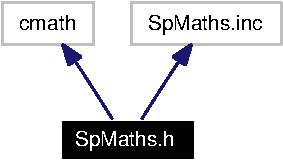
\includegraphics[width=85pt]{SpMaths_8h__incl}
\end{center}
\end{figure}


This graph shows which files directly or indirectly include this file:\begin{figure}[H]
\begin{center}
\leavevmode
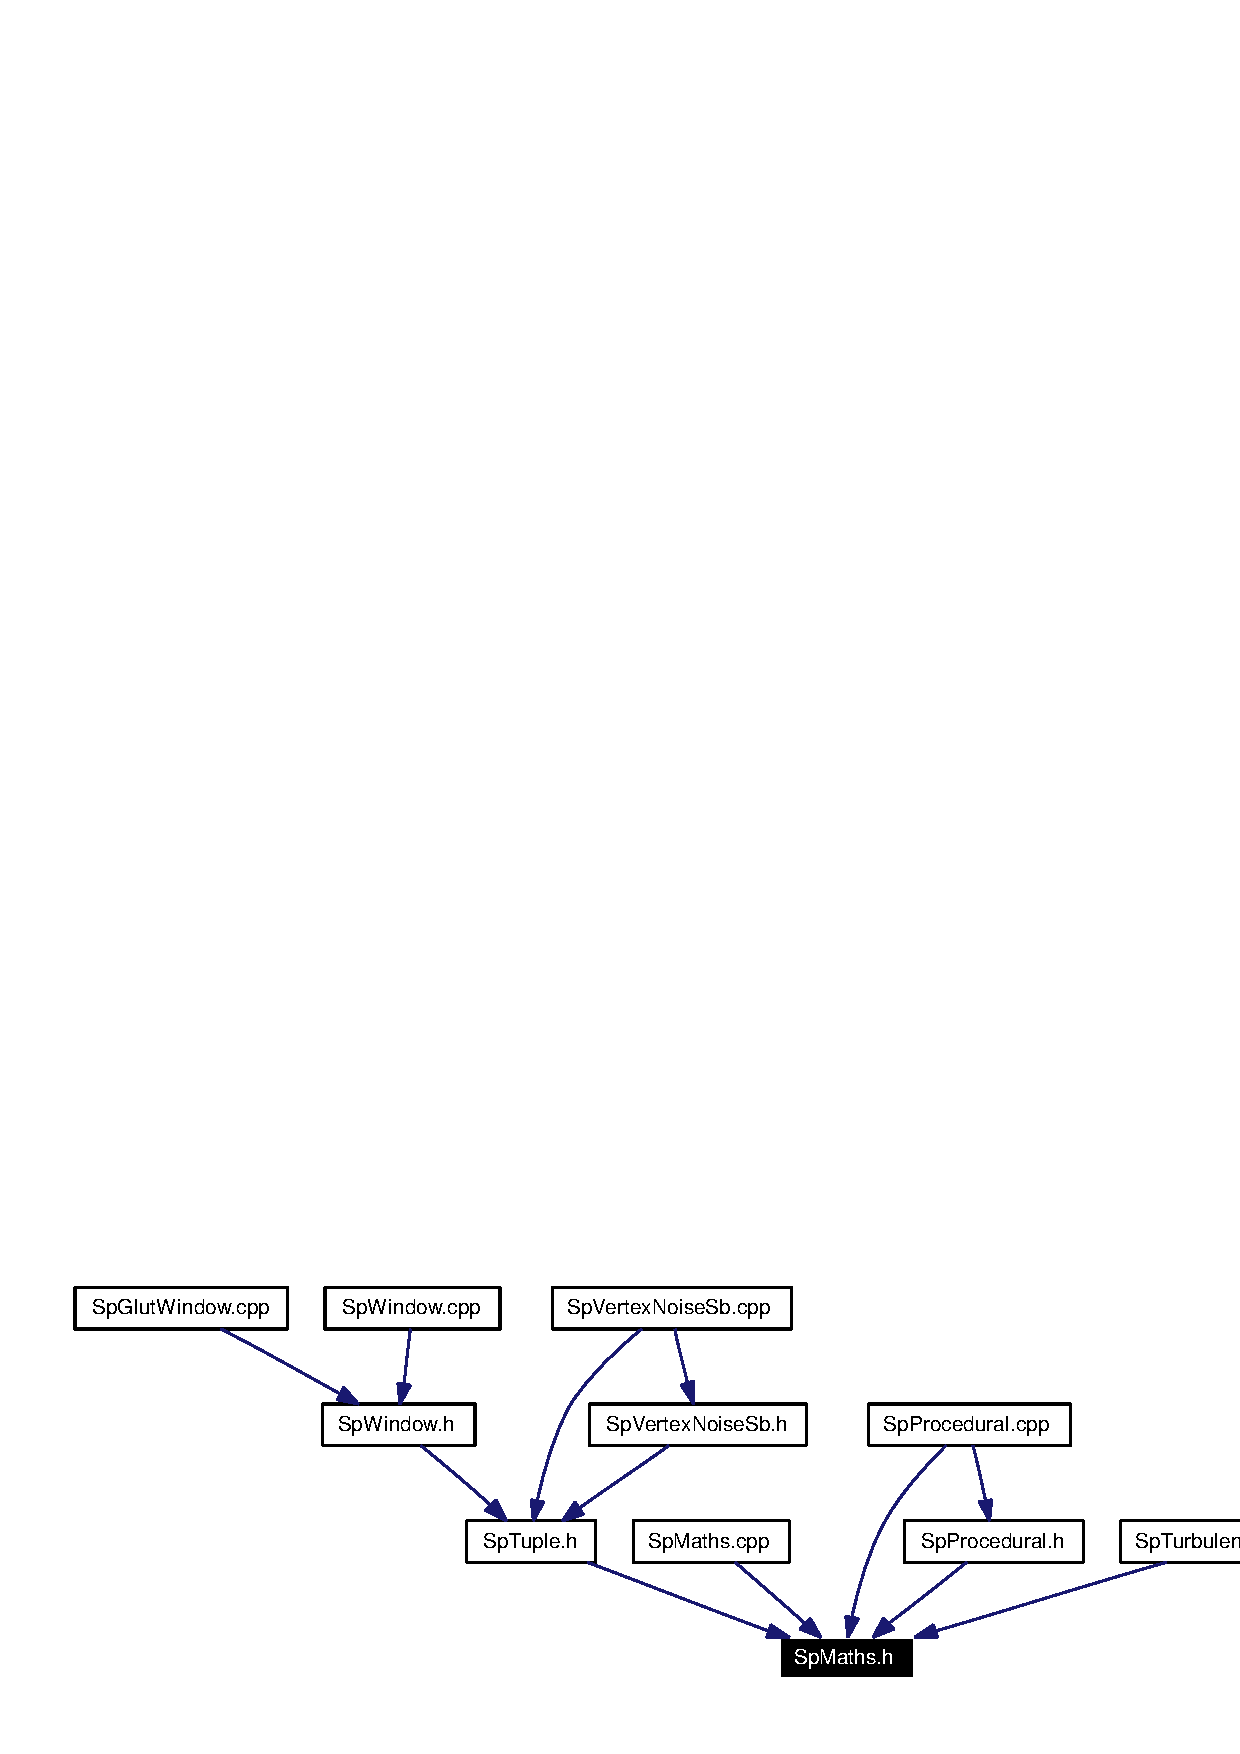
\includegraphics[width=324pt]{SpMaths_8h__dep__incl}
\end{center}
\end{figure}
\subsection*{Namespaces}
\begin{CompactItemize}
\item 
namespace {\bf Spark}
\end{CompactItemize}
\subsection*{Classes}
\begin{CompactItemize}
\item 
class {\bf Spark::Sp\-Maths$<$ Real $>$}
\begin{CompactList}\small\item\em Static utility class for mathematical constants. \item\end{CompactList}\end{CompactItemize}
\subsection*{Defines}
\begin{CompactItemize}
\item 
\#define {\bf INFINITY}\ FLT\_\-MAX
\end{CompactItemize}
\subsection*{Functions}
\begin{CompactItemize}
\item 
template$<$class Real$>$ Real {\bf Erfc} (Real f\-X)
\item 
template$<$class Real$>$ Real {\bf Log\-Gamma} (Real f\-X)
\item 
template$<$class Real$>$ Real {\bf Radians} (Real f\-Deg)
\item 
template$<$class Real$>$ Real {\bf Degrees} (Real f\-Rad)
\item 
template$<$class Real$>$ Real {\bf Abs} (Real f\-Value)
\item 
template$<$class Real$>$ Real {\bf Ceil} (Real f\-Value)
\item 
template$<$class Real$>$ Real {\bf Clamp} (Real f\-V, Real f\-Min, Real f\-Max)
\item 
template$<$class Real$>$ Real {\bf Exp} (Real f\-Value)
\item 
template$<$class Real$>$ Real {\bf Floor} (Real f\-Value)
\item 
template$<$class Real$>$ Real {\bf Inv\-Sqrt} (Real f\-Value)
\item 
template$<$class Real$>$ Real {\bf Log} (Real f\-Value)
\item 
template$<$class Real$>$ Real {\bf Pow} (Real f\-Base, Real f\-Exponent)
\item 
template$<$class Real$>$ Real {\bf Cub} (Real f\-Value)
\item 
template$<$class Real$>$ Real {\bf Square} (Real f\-Value)
\item 
template$<$class Real$>$ Real {\bf Sqr} (Real f\-Value)
\item 
template$<$class Real$>$ Real {\bf Sqrt} (Real f\-Value)
\item 
template$<$class Real$>$ Real {\bf Sign} (Real f\-Value)
\item 
template$<$class Real$>$ Real {\bf Gamma} (Real f\-X)
\item 
template$<$class Real$>$ Real {\bf Gaussian} (Real f\-X, Real f\-Std\-Dev)
\item 
template$<$class Real$>$ Real {\bf Min} (Real f\-X, Real f\-A)
\item 
template$<$class Real$>$ Real {\bf Max} (Real f\-X, Real f\-A)
\item 
template$<$class Real$>$ Real {\bf Mod} (Real f\-X, Real f\-A)
\item 
template$<$class Real$>$ Real {\bf Frac} (const Real f\-X)
\item 
template$<$class Real$>$ Real {\bf Step} (Real f\-X, Real f\-A)
\item 
template$<$class Real$>$ Real {\bf Erf} (Real f\-X)
\item 
template$<$class Real$>$ Real {\bf Arc\-Cosine} (Real f\-Value)
\item 
template$<$class Real$>$ Real {\bf Arc\-Sine} (Real f\-Value)
\item 
template$<$class Real$>$ Real {\bf Arc\-Tangent} (Real f\-Value)
\item 
template$<$class Real$>$ Real {\bf Arc\-Tangent} (Real f\-Y, Real f\-X)
\item 
template$<$class Real$>$ Real {\bf Cosine} (Real f\-Value)
\item 
template$<$class Real$>$ Real {\bf Sine} (Real f\-Value)
\item 
template$<$class Real$>$ Real {\bf Tangent} (Real f\-Value)
\item 
bool {\bf Is\-Power\-Of\-Two} (int i\-Width, int i\-Height)
\end{CompactItemize}


\subsection{Define Documentation}
\index{SpMaths.h@{Sp\-Maths.h}!INFINITY@{INFINITY}}
\index{INFINITY@{INFINITY}!SpMaths.h@{Sp\-Maths.h}}
\subsubsection{\setlength{\rightskip}{0pt plus 5cm}\#define INFINITY\ FLT\_\-MAX}\label{SpMaths_8h_a0}


Definition at line 30 of file Sp\-Maths.h.

\subsection{Function Documentation}
\index{SpMaths.h@{Sp\-Maths.h}!Abs@{Abs}}
\index{Abs@{Abs}!SpMaths.h@{Sp\-Maths.h}}
\subsubsection{\setlength{\rightskip}{0pt plus 5cm}template$<$class Real$>$ Real Spark::Abs (Real {\em f\-Value})}\label{namespaceSpark_a40}


Definition at line 164 of file Sp\-Maths.h.

Referenced by Spark::Ridged\-Multi\-Fractal(), and Spark::Turbulence().\index{SpMaths.h@{Sp\-Maths.h}!ArcCosine@{ArcCosine}}
\index{ArcCosine@{ArcCosine}!SpMaths.h@{Sp\-Maths.h}}
\subsubsection{\setlength{\rightskip}{0pt plus 5cm}template$<$class Real$>$ Real Spark::Arc\-Cosine (Real {\em f\-Value})}\label{namespaceSpark_a61}


Definition at line 275 of file Sp\-Maths.h.\index{SpMaths.h@{Sp\-Maths.h}!ArcSine@{ArcSine}}
\index{ArcSine@{ArcSine}!SpMaths.h@{Sp\-Maths.h}}
\subsubsection{\setlength{\rightskip}{0pt plus 5cm}template$<$class Real$>$ Real Spark::Arc\-Sine (Real {\em f\-Value})}\label{namespaceSpark_a62}


Definition at line 290 of file Sp\-Maths.h.\index{SpMaths.h@{Sp\-Maths.h}!ArcTangent@{ArcTangent}}
\index{ArcTangent@{ArcTangent}!SpMaths.h@{Sp\-Maths.h}}
\subsubsection{\setlength{\rightskip}{0pt plus 5cm}template$<$class Real$>$ Real Spark::Arc\-Tangent (Real {\em f\-Y}, Real {\em f\-X})}\label{namespaceSpark_a64}


Definition at line 310 of file Sp\-Maths.h.\index{SpMaths.h@{Sp\-Maths.h}!ArcTangent@{ArcTangent}}
\index{ArcTangent@{ArcTangent}!SpMaths.h@{Sp\-Maths.h}}
\subsubsection{\setlength{\rightskip}{0pt plus 5cm}template$<$class Real$>$ Real Spark::Arc\-Tangent (Real {\em f\-Value})}\label{namespaceSpark_a63}


Definition at line 305 of file Sp\-Maths.h.\index{SpMaths.h@{Sp\-Maths.h}!Ceil@{Ceil}}
\index{Ceil@{Ceil}!SpMaths.h@{Sp\-Maths.h}}
\subsubsection{\setlength{\rightskip}{0pt plus 5cm}template$<$class Real$>$ Real Spark::Ceil (Real {\em f\-Value})}\label{namespaceSpark_a41}


Definition at line 169 of file Sp\-Maths.h.\index{SpMaths.h@{Sp\-Maths.h}!Clamp@{Clamp}}
\index{Clamp@{Clamp}!SpMaths.h@{Sp\-Maths.h}}
\subsubsection{\setlength{\rightskip}{0pt plus 5cm}template$<$class Real$>$ Real Spark::Clamp (Real {\em f\-V}, Real {\em f\-Min}, Real {\em f\-Max})}\label{namespaceSpark_a42}


Definition at line 174 of file Sp\-Maths.h.

Referenced by Spark::Ridged\-Multi\-Fractal(), and Spark::Spline().\index{SpMaths.h@{Sp\-Maths.h}!Cosine@{Cosine}}
\index{Cosine@{Cosine}!SpMaths.h@{Sp\-Maths.h}}
\subsubsection{\setlength{\rightskip}{0pt plus 5cm}template$<$class Real$>$ Real Spark::Cosine (Real {\em f\-Value})}\label{namespaceSpark_a65}


Definition at line 315 of file Sp\-Maths.h.\index{SpMaths.h@{Sp\-Maths.h}!Cub@{Cub}}
\index{Cub@{Cub}!SpMaths.h@{Sp\-Maths.h}}
\subsubsection{\setlength{\rightskip}{0pt plus 5cm}template$<$class Real$>$ Real Spark::Cub (Real {\em f\-Value})}\label{namespaceSpark_a48}


Definition at line 204 of file Sp\-Maths.h.\index{SpMaths.h@{Sp\-Maths.h}!Degrees@{Degrees}}
\index{Degrees@{Degrees}!SpMaths.h@{Sp\-Maths.h}}
\subsubsection{\setlength{\rightskip}{0pt plus 5cm}template$<$class Real$>$ Real Degrees (Real {\em f\-Rad})}\label{namespaceSpark_a39}


Definition at line 69 of file Sp\-Maths.h.\index{SpMaths.h@{Sp\-Maths.h}!Erf@{Erf}}
\index{Erf@{Erf}!SpMaths.h@{Sp\-Maths.h}}
\subsubsection{\setlength{\rightskip}{0pt plus 5cm}template$<$class Real$>$ Real Spark::Erf (Real {\em f\-X})}\label{namespaceSpark_a60}


Definition at line 270 of file Sp\-Maths.h.\index{SpMaths.h@{Sp\-Maths.h}!Erfc@{Erfc}}
\index{Erfc@{Erfc}!SpMaths.h@{Sp\-Maths.h}}
\subsubsection{\setlength{\rightskip}{0pt plus 5cm}template$<$class Real$>$ Real Erfc (Real {\em f\-X})}\label{namespaceSpark_a36}


\index{SpMaths.h@{Sp\-Maths.h}!Exp@{Exp}}
\index{Exp@{Exp}!SpMaths.h@{Sp\-Maths.h}}
\subsubsection{\setlength{\rightskip}{0pt plus 5cm}template$<$class Real$>$ Real Spark::Exp (Real {\em f\-Value})}\label{namespaceSpark_a43}


Definition at line 179 of file Sp\-Maths.h.\index{SpMaths.h@{Sp\-Maths.h}!Floor@{Floor}}
\index{Floor@{Floor}!SpMaths.h@{Sp\-Maths.h}}
\subsubsection{\setlength{\rightskip}{0pt plus 5cm}template$<$class Real$>$ Real Spark::Floor (Real {\em f\-Value})}\label{namespaceSpark_a44}


Definition at line 184 of file Sp\-Maths.h.

Referenced by Spark::Cell\-Noise(), Spark::Gradient\-Noise(), and Spark::Voronoi\-Noise().\index{SpMaths.h@{Sp\-Maths.h}!Frac@{Frac}}
\index{Frac@{Frac}!SpMaths.h@{Sp\-Maths.h}}
\subsubsection{\setlength{\rightskip}{0pt plus 5cm}template$<$class Real$>$ Real Spark::Frac (const Real {\em f\-X})}\label{namespaceSpark_a58}


Definition at line 265 of file Sp\-Maths.h.\index{SpMaths.h@{Sp\-Maths.h}!Gamma@{Gamma}}
\index{Gamma@{Gamma}!SpMaths.h@{Sp\-Maths.h}}
\subsubsection{\setlength{\rightskip}{0pt plus 5cm}template$<$class Real$>$ Real Spark::Gamma (Real {\em f\-X})}\label{namespaceSpark_a53}


Definition at line 235 of file Sp\-Maths.h.\index{SpMaths.h@{Sp\-Maths.h}!Gaussian@{Gaussian}}
\index{Gaussian@{Gaussian}!SpMaths.h@{Sp\-Maths.h}}
\subsubsection{\setlength{\rightskip}{0pt plus 5cm}template$<$class Real$>$ Real Spark::Gaussian (Real {\em f\-X}, Real {\em f\-Std\-Dev})}\label{namespaceSpark_a54}


Definition at line 240 of file Sp\-Maths.h.\index{SpMaths.h@{Sp\-Maths.h}!InvSqrt@{InvSqrt}}
\index{InvSqrt@{InvSqrt}!SpMaths.h@{Sp\-Maths.h}}
\subsubsection{\setlength{\rightskip}{0pt plus 5cm}template$<$class Real$>$ Real Spark::Inv\-Sqrt (Real {\em f\-Value})}\label{namespaceSpark_a45}


Definition at line 189 of file Sp\-Maths.h.\index{SpMaths.h@{Sp\-Maths.h}!IsPowerOfTwo@{IsPowerOfTwo}}
\index{IsPowerOfTwo@{IsPowerOfTwo}!SpMaths.h@{Sp\-Maths.h}}
\subsubsection{\setlength{\rightskip}{0pt plus 5cm}bool Spark::Is\-Power\-Of\-Two (int {\em i\-Width}, int {\em i\-Height})\hspace{0.3cm}{\tt  [inline]}}\label{namespaceSpark_a68}


Definition at line 330 of file Sp\-Maths.h.\index{SpMaths.h@{Sp\-Maths.h}!Log@{Log}}
\index{Log@{Log}!SpMaths.h@{Sp\-Maths.h}}
\subsubsection{\setlength{\rightskip}{0pt plus 5cm}template$<$class Real$>$ Real Spark::Log (Real {\em f\-Value})}\label{namespaceSpark_a46}


Definition at line 194 of file Sp\-Maths.h.\index{SpMaths.h@{Sp\-Maths.h}!LogGamma@{LogGamma}}
\index{LogGamma@{LogGamma}!SpMaths.h@{Sp\-Maths.h}}
\subsubsection{\setlength{\rightskip}{0pt plus 5cm}template$<$class Real$>$ Real Log\-Gamma (Real {\em f\-X})}\label{namespaceSpark_a37}


\index{SpMaths.h@{Sp\-Maths.h}!Max@{Max}}
\index{Max@{Max}!SpMaths.h@{Sp\-Maths.h}}
\subsubsection{\setlength{\rightskip}{0pt plus 5cm}template$<$class Real$>$ Real Spark::Max (Real {\em f\-X}, Real {\em f\-A})}\label{namespaceSpark_a56}


Definition at line 260 of file Sp\-Maths.h.\index{SpMaths.h@{Sp\-Maths.h}!Min@{Min}}
\index{Min@{Min}!SpMaths.h@{Sp\-Maths.h}}
\subsubsection{\setlength{\rightskip}{0pt plus 5cm}template$<$class Real$>$ Real Spark::Min (Real {\em f\-X}, Real {\em f\-A})}\label{namespaceSpark_a55}


Definition at line 255 of file Sp\-Maths.h.\index{SpMaths.h@{Sp\-Maths.h}!Mod@{Mod}}
\index{Mod@{Mod}!SpMaths.h@{Sp\-Maths.h}}
\subsubsection{\setlength{\rightskip}{0pt plus 5cm}template$<$class Real$>$ Real Spark::Mod (Real {\em f\-X}, Real {\em f\-A})}\label{namespaceSpark_a57}


Definition at line 245 of file Sp\-Maths.h.\index{SpMaths.h@{Sp\-Maths.h}!Pow@{Pow}}
\index{Pow@{Pow}!SpMaths.h@{Sp\-Maths.h}}
\subsubsection{\setlength{\rightskip}{0pt plus 5cm}template$<$class Real$>$ Real Spark::Pow (Real {\em f\-Base}, Real {\em f\-Exponent})}\label{namespaceSpark_a47}


Definition at line 199 of file Sp\-Maths.h.

Referenced by Spark::Sp\-Turbulence\-Op::initialize().\index{SpMaths.h@{Sp\-Maths.h}!Radians@{Radians}}
\index{Radians@{Radians}!SpMaths.h@{Sp\-Maths.h}}
\subsubsection{\setlength{\rightskip}{0pt plus 5cm}template$<$class Real$>$ Real Radians (Real {\em f\-Deg})}\label{namespaceSpark_a38}


Definition at line 66 of file Sp\-Maths.h.\index{SpMaths.h@{Sp\-Maths.h}!Sign@{Sign}}
\index{Sign@{Sign}!SpMaths.h@{Sp\-Maths.h}}
\subsubsection{\setlength{\rightskip}{0pt plus 5cm}template$<$class Real$>$ Real Spark::Sign (Real {\em f\-Value})}\label{namespaceSpark_a52}


Definition at line 224 of file Sp\-Maths.h.\index{SpMaths.h@{Sp\-Maths.h}!Sine@{Sine}}
\index{Sine@{Sine}!SpMaths.h@{Sp\-Maths.h}}
\subsubsection{\setlength{\rightskip}{0pt plus 5cm}template$<$class Real$>$ Real Spark::Sine (Real {\em f\-Value})}\label{namespaceSpark_a66}


Definition at line 320 of file Sp\-Maths.h.\index{SpMaths.h@{Sp\-Maths.h}!Sqr@{Sqr}}
\index{Sqr@{Sqr}!SpMaths.h@{Sp\-Maths.h}}
\subsubsection{\setlength{\rightskip}{0pt plus 5cm}template$<$class Real$>$ Real Spark::Sqr (Real {\em f\-Value})}\label{namespaceSpark_a50}


Definition at line 214 of file Sp\-Maths.h.\index{SpMaths.h@{Sp\-Maths.h}!Sqrt@{Sqrt}}
\index{Sqrt@{Sqrt}!SpMaths.h@{Sp\-Maths.h}}
\subsubsection{\setlength{\rightskip}{0pt plus 5cm}template$<$class Real$>$ Real Spark::Sqrt (Real {\em f\-Value})}\label{namespaceSpark_a51}


Definition at line 219 of file Sp\-Maths.h.

Referenced by Spark::Quadric(), and Spark::Voronoi\-Noise().\index{SpMaths.h@{Sp\-Maths.h}!Square@{Square}}
\index{Square@{Square}!SpMaths.h@{Sp\-Maths.h}}
\subsubsection{\setlength{\rightskip}{0pt plus 5cm}template$<$class Real$>$ Real Spark::Square (Real {\em f\-Value})}\label{namespaceSpark_a49}


Definition at line 209 of file Sp\-Maths.h.\index{SpMaths.h@{Sp\-Maths.h}!Step@{Step}}
\index{Step@{Step}!SpMaths.h@{Sp\-Maths.h}}
\subsubsection{\setlength{\rightskip}{0pt plus 5cm}template$<$class Real$>$ Real Spark::Step (Real {\em f\-X}, Real {\em f\-A})}\label{namespaceSpark_a59}


Definition at line 306 of file Sp\-Procedural.h.\index{SpMaths.h@{Sp\-Maths.h}!Tangent@{Tangent}}
\index{Tangent@{Tangent}!SpMaths.h@{Sp\-Maths.h}}
\subsubsection{\setlength{\rightskip}{0pt plus 5cm}template$<$class Real$>$ Real Spark::Tangent (Real {\em f\-Value})}\label{namespaceSpark_a67}


Definition at line 325 of file Sp\-Maths.h.